\section{Representation Learning for Outlier Detection}\label{sec:representation_learning}
Shenkar and Wolf propose a contemporary framework for outlier detection that integrates representation learning with contrastive objectives. 
Within an autoencoder architecture, the method transforms input data to extract influential features for outlier detection. 
To establish the theoretical foundation for the experimental design detailed in Chapter \ref{sec:setup}, the primary paradigms of machine learning are first presented. 
Subsequently, the conceptual basis for InterCont is established through a concise explanation of the core components of contrastive learning.


Machine learning paradigms serve as overarching frameworks for interpreting data \citep[p. 4]{sarker2021machine}, providing the foundational logic for how algorithms process information. 
While individual algorithms act as specific components, the paradigm defines the broader strategy for learning. 
Consequently, many methods can be adapted across different paradigms depending on the data structure and the intended objective. 
Traditionally, the field is categorized into three primary paradigms: supervised learning, unsupervised learning, and semi-supervised learning. 
However, numerous specialized subtypes exist, such as reinforcement learning, multi-label, and transfer learning.
To establish the necessary technical background, it is essential to categorize the traditional learning frameworks and identify the specific paradigm utilized by this method. 


Supervised learning is the most widely utilized paradigm, primarily employed for classification and regression tasks. 
It relies on labeled datasets, where a model learns a mapping from inputs to specific targets \citep{lecun2015deep}. 
In this task-driven approach, the model is trained on labeled data, where each input is paired with the ground truth \citep[p.3]{sarker2021machine}. 
The model's objective is to learn a mapping function that can accurately predict labels for new, unseen data. 
While this paradigm achieves high performance for defined tasks, it is constrained by the high cost of manual data labeling and a tendency to struggle with out-of-distribution data. 


In contrast, unsupervised learning is a data-driven approach that utilizes unlabeled data by identifying underlying patterns in data without explicit labels, making it highly scalable but often less precise for specific classification tasks.
Without predefined output labels or external supervision, the model must explore the data to discover hidden patterns, underlying structures, or natural groupings \citep[p.4]{sarker2021machine}. 
This paradigm is highly scalable and effective for identifying complex relationships within large volumes of data without the need for expensive human annotation. 
However, because there are no ground truth labels to measure against, these models can be less accurate than supervised versions, and their results are often more difficult to interpret and computationally intensive.


Semi-supervised learning utilizes labeled data in conjunction with unlabeled data.
The primary objective is to leverage the structural information inherent in the unlabeled samples to improve the model's generalization performance beyond what could be achieved using the labeled data alone.
This approach is particularly valuable in scientific research where acquiring labeled instances is costly, while unlabeled data is readily available. 
By assuming that data points in close proximity share the same label, semi-supervised algorithms can propagate information from the labeled subset to the unlabeled majority, thereby refining the decision boundaries of the model.


The authors of InterCont characterize their method within the self-supervised learning paradigm \citep[p. 3]{shenkar2022anomaly}. 
This approach generates its own supervisory signals from the data structure itself \citep{jaiswal2020survey}. 
Nevertheless, the network is trained on 50\% labeled normal data and tested on the other 50\% of data that includes all labeled outliers.
For this study, the same experimental setup will be implemented for the benchmark methods.
In the proceeding thesis, this will be named semi-supervised.   


\subsection{Neural Networks}
Artificial neural networks (NN) are computational models, designed to handle tasks such as classification, pattern recognition, and predictive modeling. 
A core objective in developing these networks is to achieve high generalization \citep[p. 1]{zhang2021understanding}, ensuring that the model performs accurately on unseen test data.


The architecture of a neural network is composed of layers. 
The input layer receives raw data, where each node corresponds to a specific feature of the dataset. 
The data then progresses through one or more hidden layers.
Networks with a single hidden layer are considered shallow, while those with multiple layers are termed deep networks. 
Deep learning \cite[p. 2]{lecun2015deep} allows for the extraction of complex patterns from high-dimensional data. 
Within these layers, connections between nodes are governed by weights, which signify the relative importance of a connection.


During training, the network's output is evaluated against the ground truth using a loss function \citep{terven2025comprehensive}. 
Common loss functions include Mean Squared Error (MSE), Mean Absolute Error (MAE) or  Mean Absolute Percentage Error (MAPE) \cite[p. 6]{hassanat2024novel}. 
To minimize this loss, the model employs backpropagation \cite[p. 1]{rumelhart1986learning}. 
By applying the chain rule, the model calculates the gradient, hence the partial derivative of the loss function with respect to each weight. 
An optimizer then uses these gradients to update the parameters in the direction that reduces error. 
A single pass through the entire training dataset is referred to as an epoch. 


Activation functions \citep[p. 311]{sharma2017activation} are essential for introducing non-linearity into the model, allowing it to approximate complex functions. 
For a network to learn through backpropagation, these functions must be differentiable. 
The architecture of the InterCont method uses Tanh and LeakyReLU activation functions.
They are defined as follows:


\begin{figure}[htbp]
    \centering
    \begin{minipage}{0.5\textwidth}
        \onehalfspacing
        \textbf{Hyperbolic Tangent (tanh)}, defined as 
        \begin{equation}
            z = \frac{e^{x} - e^{-x}}{e^{x} + e^{-x}}.
        \end{equation} 
        This function is zero-centered with an output range of -1 to 1. 
        It is susceptible to vanishing gradients.
    \end{minipage}
    \hfill 
    \begin{minipage}{0.45\textwidth}
        \centering
        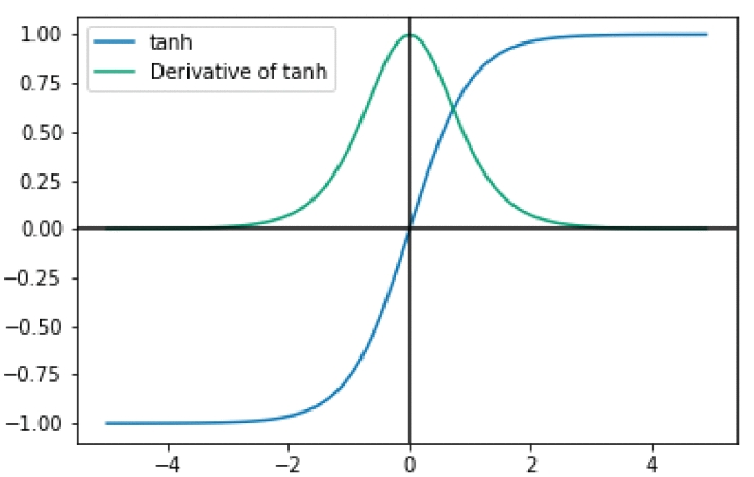
\includegraphics[width=\textwidth]{Images/Tanh}
        \vspace{0.1cm} 
        {\color{gray}\fontsize{7pt}{8pt}\selectfont Source: \citep[Fig.~4]{rasamoelina2020review}}
        \vspace{0.2cm}
        \caption{Hyperbolic Tangent Activation Function.}
    \end{minipage}
    \label{fig:tanh}
\end{figure}

\begin{figure}[htbp]
    \centering
    \begin{minipage}{0.5\textwidth}
        \textbf{Rectified Linear Unit (ReLU)}, defined as:
        \begin{equation*}
            z = \max(0, x).
        \end{equation*} 
        ReLU addresses the vanishing gradient problem by maintaining a constant gradient of 1 for all positive inputs. 
        To prevent dying ReLU, where nodes become permanently inactive due to negative inputs,
        variants like LeakyReLU are used, which allow a small, non-zero gradient for negative values.
    \end{minipage}
    \hfill 
    \begin{minipage}{0.45\textwidth}
        \centering
        \includegraphics[width=\textwidth]{Images/ReLU}
        \vspace{0.1cm} 
        {\color{gray}\fontsize{7pt}{8pt}\selectfont Source: \citep[Fig.~6]{rasamoelina2020review}}
        \vspace{0.2cm}
        \caption{ReLU Activation Function.}
    \end{minipage}
\end{figure}

\begin{figure}[htbp]
    \centering
    \begin{minipage}{0.5\textwidth}
        \onehalfspacing
        A primary challenge in training is the bias-variance tradeoff \citep[p. 14]{geman1992neural}. 
        Underfitting (high bias) occurs when a model is too simple to capture the underlying data patterns. 
        Overfitting (high variance) occurs when a model is overly complex and learns the stochastic noise of the training data rather than the generalizable signal. %\todo{more information}
        Techniques to mitigate these issues include increasing data volume, implementing dropout layers, or using early stopping to maintain the optimal balance between bias and variance.
    \end{minipage}
    \hfill 
    \begin{minipage}{0.45\textwidth}
        \centering
        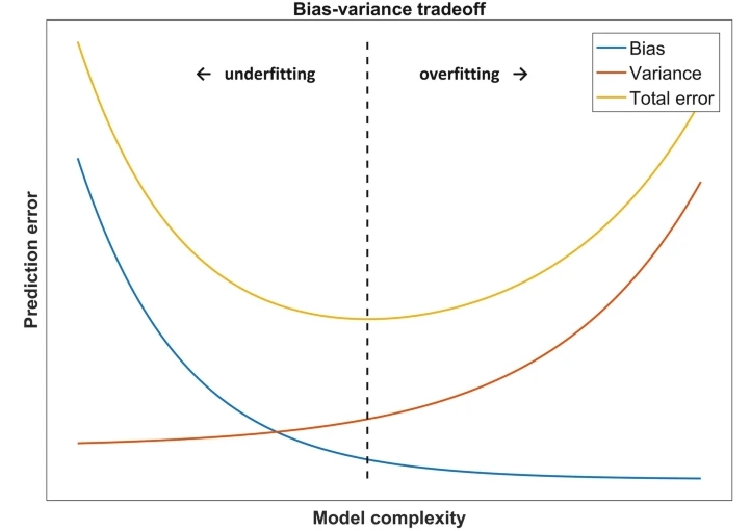
\includegraphics[width=\textwidth]{Images/Bias_Variance_Tradeoff.pdf}
        \vspace{0.1cm} 
        {\color{gray}\fontsize{7pt}{8pt}\selectfont Source: \citep[Fig.~8.3]{dankers2018prediction}}
        \vspace{0.2cm}
        \caption{Bias-Variance Tradeoff.}
    \end{minipage}
    \label{fig:bias_variance}
\end{figure}
